\documentclass[a4paper]{article}

\usepackage[english]{babel}
\usepackage[T1]{fontenc}
\usepackage{blindtext}
\usepackage[utf8]{inputenc}
\usepackage{graphicx} 
\usepackage{array}
\usepackage{verbatim}
\usepackage{hyperref}
\usepackage{subcaption}
\usepackage[acronym, toc]{glossaries}
\usepackage[dvipsnames]{xcolor}
\usepackage{caption}
\usepackage[titletoc, title]{appendix}
\usepackage{float}

\makeglossaries
\newacronym{ide}{IDE}{Integrated Development Environment}

\newacronym{md-407}{MD-407}{En ARM-baserad laborationsdator för utbildning}

\title{\textbf{Halo}\\ \large A CO2 calculator for food\\TKDAT - DAT257 / DIT257}
\author{Joar Forsberg, Sebastian Hermansson, Aziz Ibrahim \and Johan Jiremalm, Malte Landgren, Jakob Ståhl}

\date{\today}


\begin{document}
% Inga sidnumreringar här
\pagenumbering{gobble}

\maketitle
\newpage

\tableofcontents
\newpage

% Börja med sidnumrering
\pagenumbering{arabic}
 
\newpage
\section{What we have done (A)}
We are currently facing climate changes more rapidly than ever seen before in Earth’s history. The main driver of this change is human activity. The entire world’s food system accounts for one quarter of the world's greenhouse gas emissions. Of this quarter the supply chains (retailing, packaging, refrigeration, etc.) account for 18\%, and the remaining 82\% are accounted for by food production either directly (livestock, fisheries, crops for human consumption, etc.) or indirectly (land use, crops for animal consumption, etc.)\cite{FoodStat}. The purpose of this project is to make this data more readily available for consumers so as to enable them to make more climate friendly choices in their diets. 

This is accomplished by creating a website that lets the user search a database of food items and their equivalent carbon dioxide emissions. The user can then observe their emissions (represented as a pie graph or, numerically, in units of total carbon dioxide equivalent kilos) and compare the emissions of different food items. 


\newpage
\subsection{Design decisions and product structure}

Before the project started, the group was given a task to create an application that was related to one of the UNs goals. Furthermore, the application was also supposed to use an open data source of some sort. However, the form of the application was not decided, which meant the team had a lot of creative freedom. 

The team decided to create a website because it was something they had never done before, we thought it would be a good learning experience, and would be the most efficient way of creating customer value to a broad group. We then decided that the website would provide value to its users by displaying info about how their food consumption affects the climate in terms of CO2 emissions. This decision was partially made from an idea found on another website which did a similar thing if you shopped in their online store. Another reason was that we were able to find a good database which could be used for our idea\cite{Data}.

Continually, the group decided to use “React” because someone in the group had heard that it was good and that it had plenty of resources and ways to learn the framework which would increase our efficiency at creating customer value. Also, no one had ever programmed in React, javascript, html, or CSS before so we thought it would be a good learning experience. The workspace was then located in github as the group had positive prior experiences with it.


\subsection{Customer Value and Scope}
We have mainly based the project on the sustainable development goal 13 (climate action) but also targeted number 2 (zero hunger)\cite{UN}. With our website, users can see how much the food they eat impacts the world by the total CO2 emissions. There is also a dedicated page for donating to a food organization and here we chose to redirect the user to the World Food Programme as it is one of the biggest organisations that is working for this cause. The purpose of the application is to allow the user to increase their awareness on how much CO2 emissions the different foods are releasing into the environment and perhaps lower their consumption of these foods or choose other alternatives.
The main features we wanted the website to have to achieve these goals were:
\begin{itemize}
\item A food list that has a variety of foods, including the most common foods that people consume and have in their pantry such as red meat, egg, flour and sugar. 
\item Color coded CO2 emissions of each food depending on how high it is. 
\item A search bar where the user can search for a food instead of scrolling in the list. 
\item Allow the user to choose the desired amount of a food.  
\item A calculator that computes the total amount of CO2 emissions of the chosen foods and presents it as a color coded bar. 
\item Additional pages where the user can learn more about the application as well as make a donation to a food organization.
\end{itemize}
\subsubsection{Sprint-By-Sprint Prioritazation}
\textbf{For the first sprint}, we had planned to create a simple template for the website, implement the database, and also create a functional search bar. As there are six persons in the team, we decided that this would be a good start since we could divide ourselves into groups of two, where one group focused more on the frontend and the other groups focused more on the backend. 

\textbf{In sprint two}, we proceeded building on what we had done in the first sprint by adding more features. The search bar got more functionality by the addition of search tags, providing additional customer value by allowing for more options to choose from. Furthermore, the item-box got implemented which now made it possible to see the chosen items as a list, as well as remove/add an item directly from the item-box. On the frontend side, the navbar was redesigned and got some added styling. The about and donate menus got more functionality by making it possible to click on them and get redirected to their respective page. 

\textbf{In sprint three}, some new implementations were made as well as more functionality was added to existing implementations. Portion-size data was added to the rest of the data, now making it possible to choose ready-made portion sizes from the database-box. A help button was added, providing information for the user on how to use the application. We discussed whether this feature was relevant or not and decided that it could bring value for some customers that aren’t very used to technology. 

\textbf{In sprint four}, the website was coming together and we decided to provide more customer value by adding a pie chart to the item-box that displays how much the CO2 emissions of each item take up from the pie chart. We also made the CO2 emissions for each food color-coded, which can give the customer an idea of what is considered low or high. In this sprint, we also started experimenting with the user interface for mobile devices to enhance the user experience for the customer. We ended up implementing a hamburger menu that is static on mobile but also shows up when the window is shrunk on desktop, as well as made some improvements on how the website displays for mobile devices. 

\textbf{During sprint five}, we managed to get third-party feedback on the website which gave us some insights on what we could add/change from the customer's experience. One point of feedback we got was that the help-button was confusing and that we could have the information displayed all the time instead of clicking on a button. However, we had different opinions about this and decided to keep the button. Another feedback we got was that the item-box and search-bar should follow the scroll, alternatively that we have the food list inside a scroll-box. We decided that having the food list inside a scroll-box would be the fastest implementation and make the use of the website faster for the customer. A discussion we had in the previous sprint was that the pie chart was always showing, despite the fact that the user had not added any items to the item-box. For this reason, we decided to make the pie chart collapsible, giving the customer the opportunity to use it if desired. Doing it this way also saves on screen-space which gives a better user experience on mobile. 

\textbf{During the sixth and final sprint}, we focused on bug fixes and some additional improvements that could enhance the user experience for the customer on mobile. The item-box got a feature to clear all the content in one click, which saves the user time by not needing to clear all the items one by one. Another implementation that was made was the ability to switch between the database-box and the item-box on mobile, which allows us to fit everything that can be displayed on a desktop to also fit on a small screen. Previously, it looked identical on mobile as on desktop, that is, the database-box and item-box were next to each other. This was a common complaint in the 3rd party feedback as everything was hard to see and required the user to continuously zoom in and out, so that was a great improvement. 

\textbf{To summarise this}, we have after every sprint focused more and more on what implementations created value for the customer and which ones that felt redundant and could be excluded. We have tried to create value by continuously evaluating our work with the application and testing it as much as possible. Receiving third-party feedback has also been valuable as it gave us new ideas. 

\subsubsection{Success criteria for the team}
Before starting this project, we did not have any experience with agile development so our main goal with the success criteria was to learn agile development and continuously apply it during the project, as well as be able to deliver a product that we had a vision of at the end of the course.  

Another thing we wanted to achieve was becoming better working in React\cite{React} as well as the languages HTML\cite{HTML}, CSS\cite{CSS} and JavaScript\cite{JavaScript}. Pretty much none of us had any previous experience with these things, at least nothing worth talking about.

\subsubsection{User Stories}
In the first sprint we did not really write our user stories as user stories because we just interpreted the word “user story” as a general description of something to be done, and not \emph{who} is gaining value from the user story. During our first sprint-review we had a discussion about this and cleared up the confusion. Going onwards, we went from our simple user stories to begin writing user stories in the form “As a X, I want Y, because of Z" (see figure \ref{fig:US}). These small details gave us a clear overview of whom we are creating value for and also made it easier to prioritize tasks.
\begin{figure}[h]
    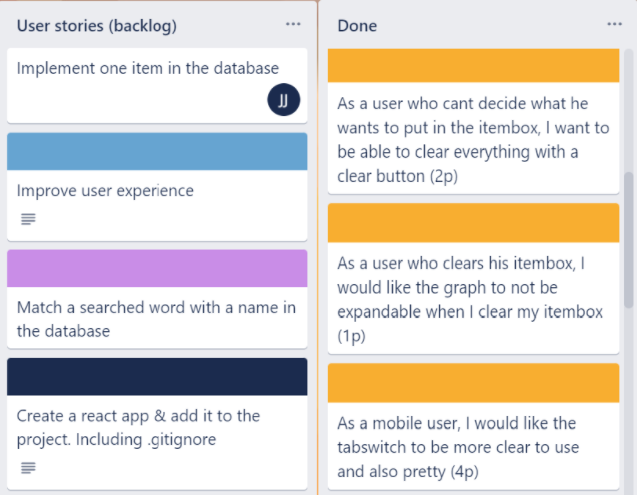
\includegraphics[width=1\textwidth]{figures/US.PNG}
    \caption{Left: Example of our user stories during the first sprint. Right: How our user stories developed going forward with the sprints and effort estimation in brackets. }
    \label{fig:US}
\end{figure}

In terms of acceptance criterias for the user stories, these were not something we made a bullet list of, but rather tried to include them in the user story itself. We think that this approach enabled us to create value, despite not being very detailed by making separate bullet lists. If we felt that we were not fully done with a user story and wanted to add more features afterwards, then we would note this for the next sprint.   
Effort estimation was also something we did not quite get into before sprint two and onwards because we were not used to writing user stories and working in an agile way. We decided that our effort estimation should be defined in terms of points. Using effort estimation gave us value by giving us an idea of the size of a user story and how much time we would need to spend working on it. Something that could be quite hard was figuring out the level of difficulty of a user story and thus underestimate the effort estimation, since we were all working with new tools and also needed some time to learn the appropriate material for that user story. 

\subsection {Social Contract and Effort}
At the start of the working process, a social contract was created with the purpose of setting up a set of rules to help the group work as a team. In particular, the contract contained information about how to handle meetings, how to divide the workload, how to handle missed deadlines, and how each member should act towards each other. These points were thoroughly discussed until the entire group was entirely satisfied with what was written in the social contract. 

Firstly, regarding the handling of meetings, it was decided that no meetings should be held before 9:15. The reason for this was that a majority of the group agreed that this would create a better activity rate during the meeting. Both because members would be less tired from waking up early, but also to give everyone some time to prepare for the meetings. Moreover, it was also decided that meetings should strive to occur during times where all of the group could participate. This was an obvious choice for us, however, it also included some limitations since we had a group with three different schedules. 

These schedules meant that the only time the entire group could partake in meetings during the workweek was on Mondays and Wednesdays which was acknowledged to be bad timings for sprint reviews since we wanted them to be at the end of the week to correlate with the end of our weekly sprints. Therefore, each meeting naturally occurred for around two hours each Sunday which was something the group was generally content with despite the contract stating that each meeting should last around 30 minutes.  

Secondly, it was decided that the group was split into three pairs which would work together on completing user stories. A list of each member’s ambition level was then created to better understand how much time each member planned on spending on the project. Time spent each week was then logged to, among other things, see how the ambition levels changed during the project. The pairs were then created considering a combination of the ambitions, together with schedule availability striving towards both being as similar as possible. The idea of working in pairs was to create an environment where getting assistance was seamless and where none would feel alone in their work. If a pair was unable to solve a certain problem, however, they were free to ask for assistance from the entire team.

In addition to working on user stories, each member was also assigned a certain area of responsibility to ensure the group kept up with the standards agreed upon. These areas included scrum master, code responsible, test responsible, and documentation responsible. The scrum master was mainly responsible for the team’s use of scrum, which included setting up and holding meetings. The code responsible’s main task was to ensure the code kept up with a set of coding standards the group agreed upon including variable names and indentations. The test responsibles were tasked with finding bugs the rest of the group was not able to find. The documentation responsibles’ task was to create a standard for documenting code and make sure each member followed this standard. However, it is worth noting that each member was responsible for following the tasks of all the areas on their own work. 

\subsection{Application of Scrum}
During the development of the website, the team used a work framework called Scrum. Scrum is a lightweight framework that helps its users generate value for its customers by continuously allowing the customer to provide feedback during the entire development process. The feedback is then being accounted for in user stories which end up in a product backlog for the developers to add. The teams then work in sprints to complete small vertical tasks that will result in something a product owner can review in the following sprint review.

Even though scrum is meant to steer the direction of the project after each sprint, it is still necessary to have a scope of what the product owner wants the project to ultimately accomplish. This was done by writing an open product scope with a base of what we thought was a minimal viable product as well as potential directions the project could take in the future. The scope was then split into a set of larger goals called epics which were used to give context to each user story. Said epics were then split among the pairs to complete the user stories connected to their appointed epic. Then each programming pair also got appointed the role as a product owner for an epic they were not responsible for delivering to simulate real product owners. However, these roles and epics were switched around a bit during the project; both because epics were replaced, and to allow new perspectives on the epics. 

Due to previously mentioned schedule conflicts the teams decided only one meeting was achievable each week. Therefore, each meeting had to include extensive information and followed a standardized agenda. The meetings started with a sprint review where each programming pair explaining what they had accomplished in each sprint followed by a dialog between the product owner and the developers where the product owners gave feedback to the developers. We felt this was a productive start to each meeting as everyone got a basic understanding on how the project had evolved and got a chance to help the team progress. 

Following the sprint review, a team reflection with weekly alternating points where the team got to reflect on the working process as a whole was held. The group generally thought this part of the meeting provided very little to no value for the team. The reason was that generally when the team had an important topic to discuss, it was brought up on the sprint review before the team reflection. Also, the questions given in the team reflection rarely fit into the topics the team thought were helpful to discuss. 

At the end of each meeting the team created user stories on trello combining the feedback provided by the product owners in the sprint review and the larger ideas in the product scope. When creating the user stories, the team tried to split the effort between each epic as evenly as possible. They were also created with the idea of fitting the INVEST criteria, and being achievable to complete within the following sprint. After the user stories had been created the team jointly gave each user story an amount of effort points depending on how much effort we thought was necessary to spend on each task. The effort points each person had ranged from 1 to 4 where 4 points would mean one person needed to work on that task for an entire week and a 1 meaning the task would take less than a day to complete. This meant that a user story with more than 4 points would be assigned to more than one person.

The process generally worked for the team, however, there were a few things that could have been improved. For instance, the effort points oftentimes did not correlate to the actual effort required to finish a task. A reason for this was that everyone was completely new to the programming environment and did not know how to do the tasks before researching them. This led to some teams finishing their weekly work in just one day at times which created productivity losses since the team could create and self-assign new user stories until the next sprint, per agile rules. Another problem the team encountered was the communication between programming pairs. Since the pairs rarely had natural communications with the entire team, all a pair could do was to either ask a question in the group chat hoping that someone would take the responsibility to help the group, or to wait until the next weekly meeting.






\newpage
\section{Discussion (A \& A->B)}
\subsection{Reflection}
The main obstacle we encountered during the project was the new technology. Since none of us had used the technology we used before, estimating tasks accurately was difficult. Oftentimes a task that was delegated a very high amount of points turned out to be trivial upon closer inspection. Similarly, tasks that were delegated a small amount of points turned out to be quite difficult. We were very quick to make our estimations. Had we been more methodical and researched our tasks more before making our estimations, they would have been more accurate. 

Of course, now that we have completed the project and we are all more experienced with the technologies that we used our estimations would have been far more accurate. But this is not exclusive to the agile process and could be said about anything. When you are learning something, the more you learn about that thing, the easier that thing becomes. So this may be a bit of a moot point. 

A more sophisticated system for handling issues would be appropriate as well. There were some issues that arose that were hard to fix. When these issues occurred, team members would have to ask other teams for help but since there was no system for describing and tracking these issues, it was harder than it should have been to reach out to other teams, describe the problem, and ask for help. We are aware that there are tools to handle this issue, such as GitHub Issues, but no such tool was used. 

The weekly meetings on Sundays where we did both the team reflections and the sprint reviews worked well for us, as opposed to having the meeting right after the sprint on Fridays evenings. It allowed us to reflect on what we’d achieved and gave us time to figure out new ideas for future implementations that we then could present for the group during the meetings. However, since it was a lot to go through in only one sitting, to have two or three shorter meetings might have made each meeting more energetic. The 3rd party-review of our project was very helpful and made us reconsider several design choices and also resulted in some new features being added. As mentioned previously some of these were not implemented but it started a discussion which was healthy. To have someone outside the working team give feedback is valuable and, looking back, it might have been rewarding to do more than once.

Regarding our use of product owners, we started by being P.O’s of our own tasks which resulted in very few questions from the rest of the group about our design choices. This was mostly for the better as it allowed us to really get into it fast which was probably necessary with the course not having so many sprints. Too many questions during the first couple of weeks could potentially lead to an unfinished product or stress later on during the project. However, after the first week, we decided to separate product owners from developers to allow for more discussion, which overall most definitely led to better code, when other people gave their opinion on your work.


\subsection{What We Have Learned As a Group}
Throughout the course of the project, the team as a whole has picked up both tool and workstyle related skills. To begin with, the team members have gained concrete skills in common programming paradigms such as JavaScript\cite{JavaScript} and the subsidiary framework “React”\cite{React}, as well as the related CSS\cite{CSS} and HTML\cite{HTML} languages. Furthermore, (although previously experienced) skills were improved with GIT and Github which were used to handle version control and host the repository. 

In the realm of more abstract skills, the team learned about the Agile work-method*. More specifically, Scrum was the Agile methodology practiced throughout the project (although with incremental and team influenced modifications). One of these modifications was originally a misunderstanding of the Scrum framework, and resulted in us defining intra-sprint MVPs. However, once this discovery was made our “sprint MVPs” had already become a beloved part of our planning process which allowed us to easily prioritize user stories. This had a lot of synergy with the agile mindset, as it led to the most integral features getting completed early in the sprint, allowing them to potentially be reviewed by a PO and revised before the official sprint review. Moreover, the “sprint MVPs” in and of themselves were a convenient summary of sprint-by-sprint progress. This aspect is something that we believe would provide value for investors/overseers not concerned with intra-sprint details, but with a birds eye view* of the progress. 

Concerning creating a good birds eye view of the project, we chose three KPIs to keep track of our progress. These KPIs were “Burndown”, “Velocity” and “Code Churn”, and are all productivity focused. Our intention was to focus on productivity to quickly get the project started, and change KPIs later if needed (in alignment with the agile work method). However, in the last half of the project, we realised the importance of diversifying the KPIs as we better understood the considerable overlap in our current lineup. We consequently added another metric, customer feedback, which quickly became the most useful datapoint in describing the state of the project in the opinion of the team. Furthermore, we learned the importance of KPI-planning* in the initial project planning stage and that it should not be glossed over to, for instance, avoid bad data points. For example, with “Code Churn” we used gitHub’s built-in* statistics page. However, it only considered commits directly to main (excluding even merges) which meant that team members with the preference of creating git branches were invisible to the KPI. 


\subsection{Goals For Future Endevours}
In a future agile project it may be useful to perform more research regarding the implementation of various features to ensure that our estimated effort for the tasks are more accurate. Likely, doing so will help in dividing tasks more evenly among the team members and thereby increase productivity.

One of the most useful tools would be to implement a system that assists people when they need help with an issue. At times during the project people requested assistance without receiving any. The problem partly stems from a lack of clarity. To request help one had to post a question in the discord chat. Whether or not the request was answered was unclear to other team participants and there was no clear structure that ensured help was given. In a future agile project this issue can be resolved by utilizing existing tools like the issue tracker in GitHub. Moreover, assigning a weekly meet up where the entire team works together and advises one another may move the project along faster and prevent pauses in productivity.

The weekly meetings for sprint reviews would be implemented again. To have these meetings a couple days after the end of a sprint worked well and could be further utilized by officially requesting that the team reflect on future improvements once they complete the sprint. Looking over the project at the end of a sprint may improve both the understanding of the current implementation as well as result in more creative ideas regarding future development. To an extent this was already done but making it an official task every sprint may yield further improved productivity. 

P.Os would be further utilized as they were very useful. Having a person to answer to regarding one's work is very important as it incentivises a better work ethic and promotes useful and understandable features. However, starting off the project as P.Os of oneselves’ user stories did quicken the pace during the first week and this would be an idea to keep in mind for future projects.

Having third party opinions (opinions from the customer) helped create a website that actually serves the customer. This will be useful in most projects where the goal is to deliver value to the customer.

Pair programming was very useful as multiple inputs on every task lead to faster development and can offload some workload. Furthermore, it is better for productivity for two people to keep track of each other and their work than to have everybody work separately as it is more difficult to then make sure that everybody is performing their assigned tasks. Also, working on the same feature parallel to one another as was sometimes done meant that when one person was taking a break, the other could revise the current progress and build upon the other person’s work. The benefits of pair programming are thereby definitely desirable to have in a future project.

Finally, the Trello board helped keep track of the work and achieved a good understanding of the project as a whole and ongoing work on individual deliverables. A board or map similar to this will be useful.





%\newpage
\addcontentsline{toc}{section}{References}
\bibliographystyle{IEEEtran}
\bibliography{references}

%\newpage
\pagenumbering{Roman}


\end{document}